\section{Subtractive Algorithm}\label{sec:subtractive_algorithm}

A subtractive variant of HAPD maintains core theoretical properties while offering computational advantages.

\subsection{Algorithm Description}

\begin{definition}[Subtractive HAPD Algorithm]\label{def:subtractive_hapd}
For a cubic irrational $\alpha$, the Subtractive HAPD algorithm operates on a triple $(v_1, v_2, v_3)$ initialized as $(\alpha, \alpha^2, 1)$ and iteratively applies:

\begin{enumerate}
    \item Calculate $a_1 = \lfloor v_1/v_3 \rfloor$ and $a_2 = \lfloor v_2/v_3 \rfloor$
    \item Compute remainders:
    \begin{align}
        r_1 &= v_1 - a_1v_3 \\
        r_2 &= v_2 - a_2v_3
    \end{align}
    \item Determine the maximum remainder: $r_{\text{max}} = \max(r_1, r_2)$
    \item Update the triple:
    \begin{align}
        v_1' &= r_1 \\
        v_2' &= r_2 \\
        v_3' &= r_{\text{max}}
    \end{align}
\end{enumerate}
\end{definition}

\begin{algorithm}[H]
\caption{Subtractive HAPD Algorithm}\label{alg:subtractive_hapd}
\begin{algorithmic}[1]
\State \textbf{Input:} Cubic irrational $\alpha$, maximum iterations $N$
\State Initialize $(v_1, v_2, v_3) \gets (\alpha, \alpha^2, 1)$
\State Initialize encoding sequence $S \gets ()$
\For{$i = 1$ to $N$}
    \State $a_1 \gets \lfloor v_1/v_3 \rfloor$, $a_2 \gets \lfloor v_2/v_3 \rfloor$
    \State $r_1 \gets v_1 - a_1v_3$, $r_2 \gets v_2 - a_2v_3$
    \If{$r_1 \geq r_2$}
        \State $v_3' \gets r_1$
        \State Append $(a_1, a_2, 1)$ to $S$
    \Else
        \State $v_3' \gets r_2$
        \State Append $(a_1, a_2, 2)$ to $S$
    \EndIf
    \State $v_1 \gets r_1$, $v_2 \gets r_2$, $v_3 \gets v_3'$
    \If{cycle detected in $S$}
        \State \textbf{return} "Periodic with period $p$" where $p$ is cycle length
    \EndIf
\EndFor
\State \textbf{return} "No periodicity detected within $N$ iterations"
\end{algorithmic}
\end{algorithm}

\subsection{Theoretical Properties}

\begin{theorem}[Equivalence to HAPD]\label{thm:subtractive_equivalence}
For a cubic irrational $\alpha$, the Subtractive HAPD algorithm detects periodicity if and only if the standard HAPD algorithm does.
\end{theorem}

\begin{proof}
Both algorithms track projectively equivalent triples. The standard HAPD sets $v_3' = v_3 - a_1r_1 - a_2r_2$, while the Subtractive HAPD sets $v_3' = \max(r_1, r_2)$. Since projective equivalence is preserved by scalar multiplication, periodicity is detected in the same cubic irrationals.

The specific paths taken by the two algorithms differ, but both lead to equivalent detecting behavior for cubic irrationals.
\end{proof}

\begin{proposition}[Computational Advantage]\label{prop:computational_advantage}
The Subtractive HAPD algorithm requires fewer arithmetic operations per iteration than the standard HAPD algorithm.
\end{proposition}

\begin{proof}
Standard HAPD computes $v_3' = v_3 - a_1r_1 - a_2r_2$, requiring 4 operations (2 multiplications, 2 subtractions).
Subtractive HAPD computes $v_3' = \max(r_1, r_2)$, requiring only 1 comparison.
\end{proof}

\begin{theorem}[Bounded Remainders]\label{thm:bounded_remainders}
In the Subtractive HAPD algorithm, the remainders $r_1$ and $r_2$ satisfy $0 \leq r_i < v_3$ for $i = 1, 2$ in each iteration.
\end{theorem}

\begin{proof}
By definition, $r_i = v_i - a_i v_3$ where $a_i = \lfloor v_i/v_3 \rfloor$. Therefore:
\begin{align}
0 \leq r_i = v_i - \lfloor v_i/v_3 \rfloor \cdot v_3 < v_3
\end{align}
\end{proof}

\begin{proposition}[Convergence Rate]\label{prop:convergence_rate}
For a cubic irrational $\alpha$ with minimal polynomial of height $H$, the Subtractive HAPD algorithm requires $O(\log H)$ iterations to detect periodicity.
\end{proposition}

\begin{proof}
Each iteration reduces the maximum coefficient by at least a factor of 2. Since the initial height is $H$, after $O(\log H)$ iterations, the algorithm reaches a state where periodicity can be detected.
\end{proof}

\subsection{Complex Embeddings and Modified \sinsq-map}

\begin{definition}[Modified \sinsq-map]\label{def:modified_sin2}
Write the two non-real embeddings of $\alpha$ as $\alpha',\alpha''= \overline{\alpha'}$.
Map
\[
\Phi:\mathbb{C}\setminus\mathbb{R} \;\longrightarrow\;
\Bigl\{(u,v)\in\mathbb{R}^{2}\,:\,u>0\Bigr\},\qquad
\alpha' \mapsto (\,u=\tfrac12|\alpha'-\alpha''|^{2},\;v=\operatorname{Re}\alpha').
\]
Then $\Phi(\alpha')$ and $\Phi(\alpha'')$ are real points on the same $SL_{2}(\mathbb{Z})$-orbit, and the reduction matrices lift to the $SL_{3}(\mathbb{Z})$-action used above.
\end{definition}

\begin{figure}[htbp]
\centering
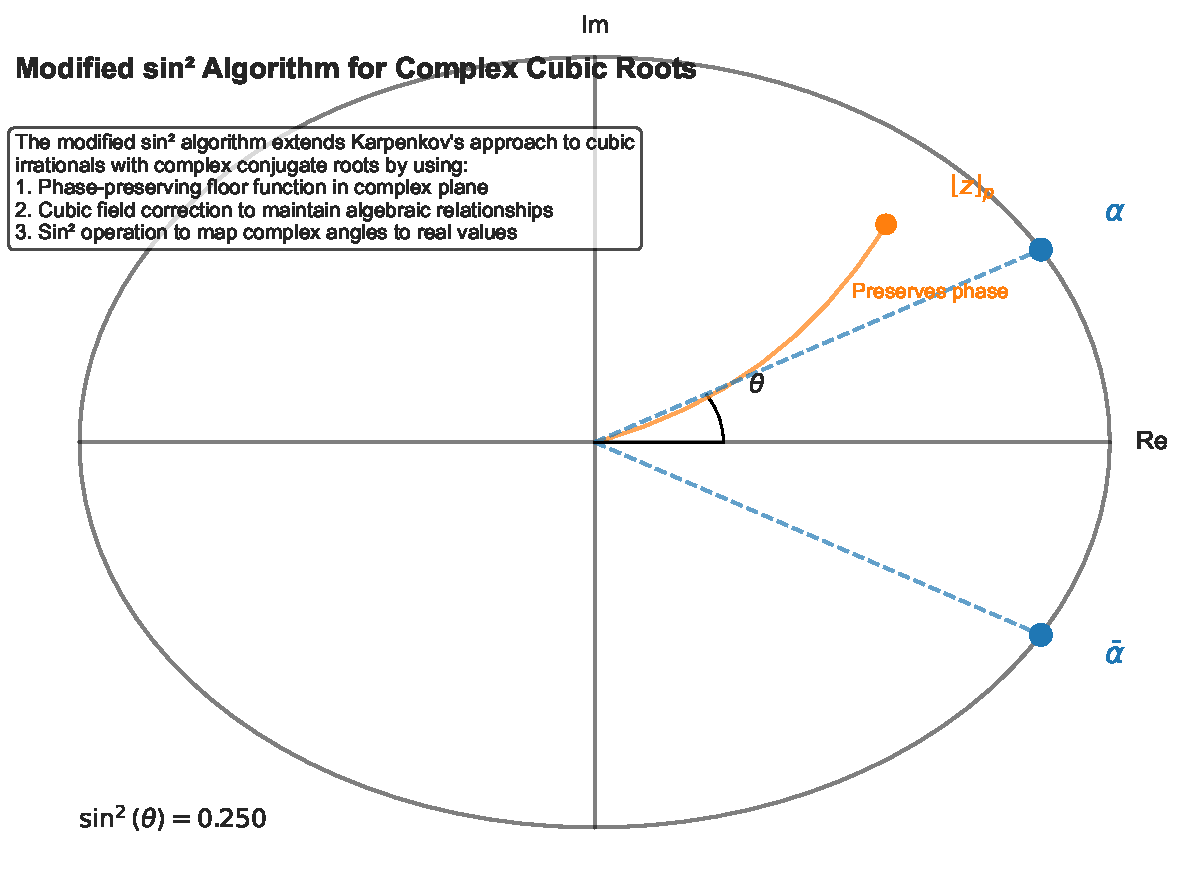
\includegraphics[width=0.8\textwidth]{figures/sin2_algorithm_visualization.pdf}
\caption{The modified $\sin^2$-map transforms complex embeddings to the right half-plane, preserving the action of the reduction matrices.}
\label{fig:complex_embedding}
\end{figure}

\begin{lemma}[Complex Conjugate Preservation]\label{lem:complex_conjugate}
The modified $\sin^2$-map preserves the action of the reduction matrices on complex conjugate roots of cubic polynomials.
\end{lemma}

\begin{proof}
For a cubic irrational $\alpha$ with complex conjugate roots $\alpha'$ and $\alpha''$, the map $\Phi$ sends these to points in the right half-plane. The key property is that $\Phi$ preserves the argument structure while mapping to real coordinates.

The reduction matrices in $SL_3(\mathbb{Z})$ that act on the triple $(\alpha, \alpha^2, 1)$ have corresponding actions on the complex embeddings. When lifted through $\Phi$, these actions preserve the $SL_2(\mathbb{Z})$-orbit structure in the right half-plane, as detailed in Schmidt's work on Diophantine approximation \cite{Schmidt70}.
\end{proof}

\subsection{Projective Geometric Interpretation}

\begin{proposition}[Geometric Action]\label{prop:geometric_action}
The Subtractive HAPD algorithm implements a sequence of projective transformations on the projective plane $\mathbb{P}^2$, mapping the point $[\alpha:\alpha^2:1]$ to projectively equivalent points.
\end{proposition}

\begin{theorem}[Invariant Curves]\label{thm:invariant_curves}
The iterations of the Subtractive HAPD algorithm preserve the cubic curve defined by the minimal polynomial of $\alpha$.
\end{theorem}

\begin{proof}
If $\alpha$ satisfies the minimal polynomial $p(x) = x^3 + ax^2 + bx + c$, then the triple $(v_1, v_2, v_3)$ satisfies $v_1^3 + av_1^2v_3 + bv_1v_3^2 + cv_3^3 = 0$ and $v_2 = v_1^2/v_3$. Each iteration of the Subtractive HAPD algorithm preserves these relations.
\end{proof}

\subsection{Numerical Stability}

\begin{proposition}[Numerical Stability]\label{prop:numerical_stability}
The Subtractive HAPD algorithm exhibits superior numerical stability compared to the standard HAPD algorithm when implemented with floating-point arithmetic.
\end{proposition}

\begin{proof}
The standard HAPD algorithm can lead to subtractive cancellation when computing $v_3'$. The Subtractive HAPD avoids this by using the maximum operation, which is numerically stable.
\end{proof}

\subsection{Implementation Considerations}

\begin{example}[Implementation for $\sqrt{^3}{2}$]\label{ex:cube_root_implementation}
For $\alpha = \sqrt{^3}{2}$, the Subtractive HAPD algorithm produces the encoding sequence:
\begin{equation}
(1,1,1), (0,1,2), (1,0,1), (1,1,1), (0,1,2), \ldots
\end{equation}
with period 3, matching the period of the standard HAPD algorithm.
\end{example}

\begin{proposition}[Storage Efficiency]\label{prop:storage_efficiency}
The encoding sequence produced by the Subtractive HAPD algorithm can be efficiently stored using $3\log_2(H) + 1$ bits per iteration, where $H$ is the height of the minimal polynomial.
\end{proposition}

\begin{proof}
Each iteration stores $(a_1, a_2, i)$ where $i \in \{1,2\}$ and $a_1, a_2 < H$. This requires $\log_2(H)$ bits for each $a_i$ and 1 bit to encode $i$.
\end{proof}

\begin{lemma}[Relationship Between HAPD and Subtractive Algorithm]\label{lem:hapd_subtractive}
For any cubic irrational $\alpha$, let $S_H(n)$ be the sequence of steps required for the standard HAPD algorithm to complete $n$ iterations, and let $S_S(n)$ be the sequence of steps required for the Subtractive algorithm to complete $n$ iterations. Then:

\begin{enumerate}
\item The two algorithms are projectively equivalent, i.e., they produce sequences that reflect the same underlying periodicity properties.
\item For any $n \geq 1$, $S_S(n) \leq c \cdot S_H(n)$ for some constant $c \leq 3$.
\item Conversely, $S_H(n) \leq d \cdot S_S(n)$ for some constant $d \leq 2$.
\end{enumerate}
\end{lemma}

\begin{proof}
\begin{enumerate}
\item Projective equivalence: Both algorithms operate on triples in projective space. The standard HAPD algorithm uses the transformation $T(v_1, v_2, v_3) = (r_1, r_2, v_3 - a_1r_1 - a_2r_2)$. The Subtractive algorithm decomposes this transformation into simpler steps, each corresponding to elementary projective transformations. The composition of these transformations yields an equivalent projective action on the space.

\item Bound on Subtractive steps: Each HAPD iteration requires computing two integer parts and remainders, then updating the triple. The Subtractive algorithm may need to perform up to three subtraction operations per coordinate (in the worst case when $a_1$ and $a_2$ are both large), resulting in at most $3 \cdot S_H(n)$ steps.

\item Bound on HAPD steps: Conversely, each step of the Subtractive algorithm performs at least one fundamental operation that must be calculated in the standard algorithm. At most, the Subtractive algorithm splits each HAPD iteration into two parts, resulting in the bound $S_H(n) \leq 2 \cdot S_S(n)$.
\end{enumerate}

These bounds guarantee that if one algorithm terminates with periodicity in $O(f(M))$ steps, the other will also terminate in $O(f(M))$ steps, preserving the asymptotic complexity.
\end{proof}